
\documentclass[11pt]{article}

\usepackage{common}
\usepackage{listings}
\usepackage[toc,page]{appendix}
\title{HW4: Word Segmentation}
\author{Virgile Audi \\ vaudi@g.harvard.edu \\ Nicolas Drizard \\ nicolasdrizard@g.harvard.edu}
\begin{document}

\maketitle{}
\section{Introduction}

The goal of this assignement is to implement reccurent neural networks for a word segmentation task. The idea is to identify the spaces in sentence based on the previous characters only. This could be particularly helpful for processing languages written without spaces such as Korean or Spanish


\section{Problem Description}

The problem that needs to be solve in this homework is the following: given a sequence of characters, predict where to insert spaces to make a valid sentence. For instance, consider the following sequence of character:
\begin{center}
I A M A STUDENT IN C S 2 8 7\\
\end{center}
the implemented algorithm should be capable of segmenting this sequence into valid words to give:
\begin{center}
I am a student in CS 287\\
\end{center}

\noindent To solve this problem, we will train different language models including count-based models, basic neural networks, and recurrent neural networks, combined with two search algorithms to predict the right position for spaces, i.e. a greedy search algorithm and the Viturbi algorithm. 


\section{Model and Algorithms}

\subsection{Count-based Model}

The first model is a count-based character n-gram model. The goal is to compute the probability of the newt word being a space:

\[ P(w_i =<\mathrm{space}> | w_{i-n+1}, \ldots w_{i-1}) \]

This model is built by computing its MLE which gives:

\[ P(w_i =<\mathrm{space}> | w_{i-n+1}, \ldots w_{i-1}) = \frac{F_{c_i,s}}{F_{c_i,.}}\]

where $c_i = w_{i-n+1}, \ldots w_{i-1}$ is the context for the word $w_i$. We add a smoothing parameter $\alpha = 0.1$ just for the rare corner cases where the context was unseen (which is really rare in comparison to count-based word level models).

\subsection{Neural Language Model}
As a second baseline, we implemented a neural language model to predict whether the next character is a space or not. The model is similar to the Bengio model coded in HW3 but is adapted to characters. Similarly to what we did for word prediction, we imbed a window of characters in a higher dimension using a look-up table. We first apply a first linear model to the higher dimensional representation of the window of characters, followed by a hyperbolic tangent layer to extract non-linear features. A second linear layer is then applied followed by a softmax to get a probability distribution over the two possible outputs, i.e. a character or a space.\\
\noindent We can summarize the model in the following formula: $$nnlm_1(x) = \tanh(\mathbf{xW}+\mathbf{b})\mathbf{W'}+\mathbf{b'}$$
where we recall:
\begin{itemize}
\item $\boldsymbol{x}\in \Re^{d_{in}\cdot d_{win}}$ is the concatenated character embeddings
\item $\boldsymbol{W}\in \Re^{(d_{in}\cdot d_{win})\times d_{hid}}$, and $\boldsymbol{b}\in \Re^{d_{hid}}$
\item $\boldsymbol{W'}\in \Re^{d_{hid}\times 2}$, and $\boldsymbol{b'}\in \Re^{2}$.
\end{itemize}


\subsection{Algorithm to generate spaces sequences}
As mentioned in the problem description, in order to predict the position of a space, we will use two search algorithm. Both of these algorithm use the language models mentioned above to predict the next character or space given the prior context.

\subsubsection{Greedy}
The greedy algorithm implemented is an algorithm that chooses the locally optimum choice at every step in the sequence. This algorithm does not generally lead to a global maxium but has the advantage of being easilly implementable and efficient both in memory and complexity. The pseudo-code of the algorithm is presented below:

 \begin{algorithmic}[1]
    \Procedure{GreedySearch}{}
    \State{s=0}
    \State{$c\in \mathcal{C}^{n+1}$}
    \State{$c_0 = \langle s \rangle$}
    \For{i = 1 to n}
    \State{Predict the distribution $\mathbf{\hat{y}}$ over the two classes given the previous context}
    \State{Pick the next class that maximises the distribution $c_i \leftarrow \arg\max\limits_{c'_i}\mathbf{\hat{y}}(c_{i-1})_{c_i}$}
    \State{Update the score of the chain: $s+\log\mathbf{\hat{y}(c_{i-1})}_{c_i}$}
    \State{Update the chain/context by adding a space or the following character}
    \EndFor{}
	\Return{the chain and the score}
    \EndProcedure{}
  \end{algorithmic}
\subsubsection{Viterbi}
The second search algorithm that we implemented is the dynamic programming algorithm named after Andrew Viterbi. The main difference with the greedy algorithm is that it evaluates at every step and for every previous state, the best possible next step. This would guarantee a solution closer to the true optimal solution. In our case of predicting character or space, the algorithm keeps track of the best sequences that could lead to a character or a space at step i-1, and then evaluates both path for both class, i.e. space to space, space to character, character to space and character to character, using the language models. It then keeps the path that has the highest score for each of the 2 states. The pseudo-code of the algorithm is given by:\\

\begin{algorithmic}
    \Procedure{ViterbiWithBP}{}
    \State{$\pi \in \reals^{ n+1 \times \mcC}$ initialized to $-\infty$ }
    \State{$bp \in \mcC^{n \times \mcC}$ initialized to $\epsilon$ }
    \State{$\pi[0, \langle s \rangle] = 0$}
    \For{$i = 1$ to $n$ }
    \For{$c_{i-1} \in \mcC$}
    \State{compute $\hat{\boldy}(c_{i-1})$}
    \For{$c_{i} \in \mcC$}
    \State{$score = \pi[i-1, c_{i-1}] + \log \hat{\boldy}(c_{i-1})_{c_i} $}
    \If{$score > \pi[i, c_i]$}
    \State{$\pi[i, c_i] = score$}
    \State{$bp[i, c_i] = c_{i-1}$}
    \EndIf{}
    \EndFor{}
    \EndFor{}
    \EndFor{}
    \State{\Return{sequence from $bp$}}
    \EndProcedure{}
  \end{algorithmic}
  
 \noindent We implemented this algorithm for both bigram, and trigram models.

\subsection{Recurrent Neural Networks}

We implemented three different recurrent neural networks and benchmark their performance in our experiments. The main point is that we want to compute one output for each timestep and not only for the last one, that's why the generic structure of our networks is a tranducer.

\paragraph{Generic RNN Transducer}

The motivation is to maintain history in the model by the introduction of hidden states at each time steps (here each character of the input sequence). The model contains two main transformation: the transition function that define the hidden state given $\mathbb{s_{i}}$ the current input $x_i$ and the previous hidden state $\mathbb{s_{i-1}}$ and the output layer producing the output $\mathbb{y_i}$ at each timestep. We used Elman tanh layer for the output.

\begin{figure}[H]
\begin{center}
    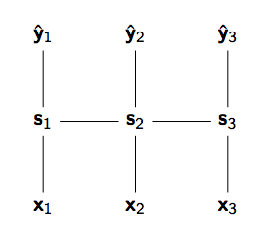
\includegraphics[width=0.45\textwidth]{transducer.png}
    \caption{Transducer Architecture}
\end{center}
\end{figure}

Formally:

\begin{align*}
\mathbb{\hat{y_i}} = softmax(\mathbb{s_i} \mathbb{W} + \mathbb{b}) \\
\mathbb{s_i} = tanh( [\mathbb{x_i}, \mathbb{s_{i-1}}\mathbb{W} + \mathbb{b})
\end{align*}

We used a batch version to learn the model and split the batched sequences in small chunks of characters of a given length to do the backpropagation to make it run faster. We explored different values for the two parameters length and batch size. 


\paragraph{GRU}

This models introduces the gating operation that allows a vector $\mathbb{t}$ to mask or gate $\mathbb{x}$. This operation is smoothed with a sigmoid: $t = \sigma(\mathbb{W^t}\mathbb{x} + \mathbb{b})$. This operation is used to stop connection by applying the reset gate $\mathbb{r}$. This operation may be useful to avoid issue with the long sequence of gradients we need to compute in the backpropagation phase.

Formally:

\begin{figure}[H]
\begin{center}
    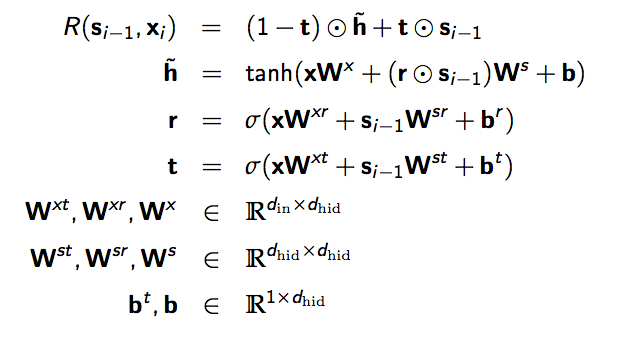
\includegraphics[width=0.45\textwidth]{gru.png}
    \caption{GRU equations}
\end{center}
\end{figure}

\paragraph{LSTM}

The long short term memory network uses also the gate idea with three gates: input, output and forget.

\begin{figure}[H]
\begin{center}
    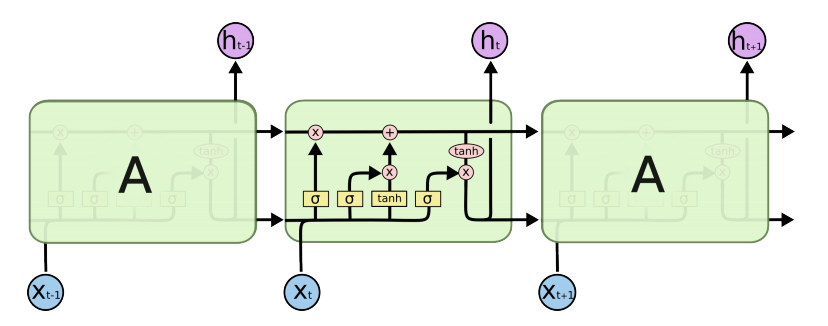
\includegraphics[width=0.45\textwidth]{lstm.png}
    \caption{LSTM Architecture}
\end{center}
\end{figure}

Formally:

\begin{figure}[H]
\begin{center}
    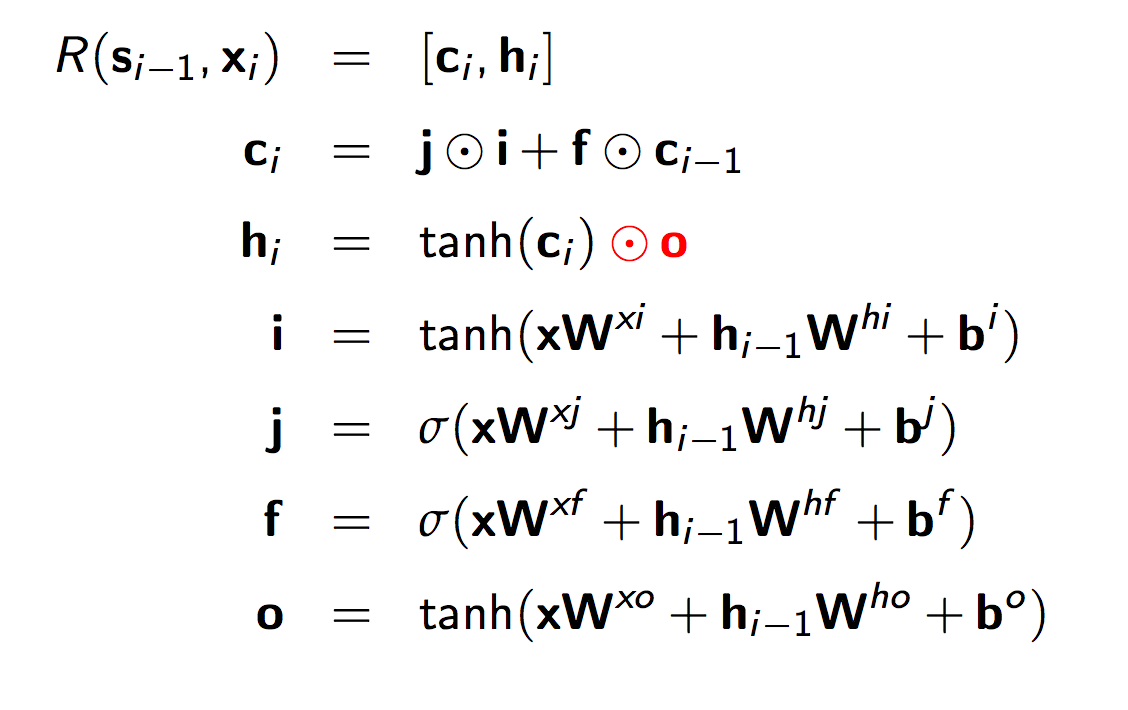
\includegraphics[width=0.45\textwidth]{lstm_eq.png}
    \caption{Perplexity evolution for the GRU}
\end{center}
\end{figure}


\section{Experiments}

\subsection{Count-based Model}

This first approach relies on a window approach where we predict the next character given a fixed size of previous character. This size is the only parameter of the model. Then, we can apply the two algorithms described to predict a sequence given our trained model. 

To evaluate the performance of the model gienve the size of the Ngram, we computed the perplexity of the training and validation data.

\begin{figure}[H]
\begin{center}
    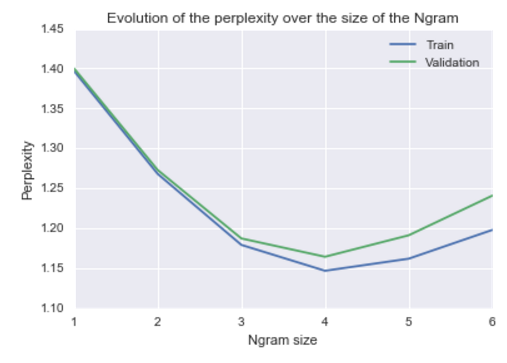
\includegraphics[width=0.45\textwidth]{count_graph.png}
    \caption{Perplexity evolution for the RNN}
\end{center}
\end{figure}

We observed an optimum of perplexity for the Ngram in both the validation and the train set. Then the steeper slope of the validation is due to overfitting. As a result, we sticked to this value for the model.\\

We implemented the greedy algorithm and the Viterbi one up to the trigram (so with a bigram as a context). Coding the Viterbi for larger Ngram size requires to cover more and more possibilities in our class $C$ (given the position of spaces in the sequence). 


\subsection{Neural Language Model}
Based on the results of the dynamic search on count-based models using bigram, we concluded that it was best to show results of the greedy algorithm with greater n-grams for the neural language model. In order to compare the results, we fixed the embedding size of the characters to 15, as well as the hidden dimension to 80 and the batch size to 20. We then train models for 3,4 and 5-grams, evaluate the loss on training, and use for validation the RMSE of the number of spaces predicted on each sentence of the validation set.\\

We present the results:

\begin{figure}[H]
\centering
\begin{minipage}{.5\textwidth}
  \centering
  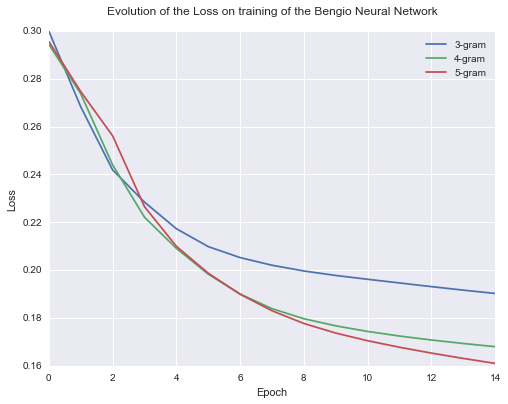
\includegraphics[width=1\linewidth]{train_nn}
  \caption{Training Loss}
\end{minipage}%
\begin{minipage}{.5\textwidth}
  \centering
  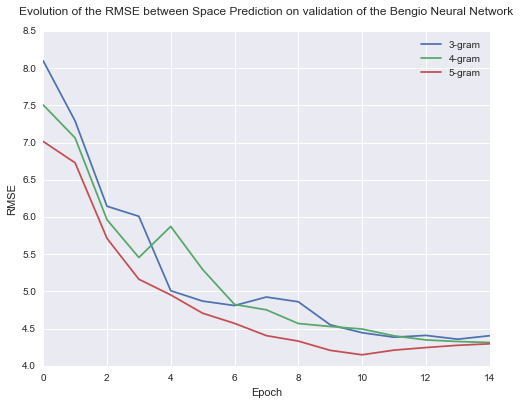
\includegraphics[width=1\linewidth]{rmse}
  \caption{RMSE on Validation set}
\end{minipage}
\end{figure}

As expected, performance increases with the size of the n-grams. We then tested the impact of the embedding size. 

\begin{figure}[H]
\centering
\begin{minipage}{.5\textwidth}
  \centering
  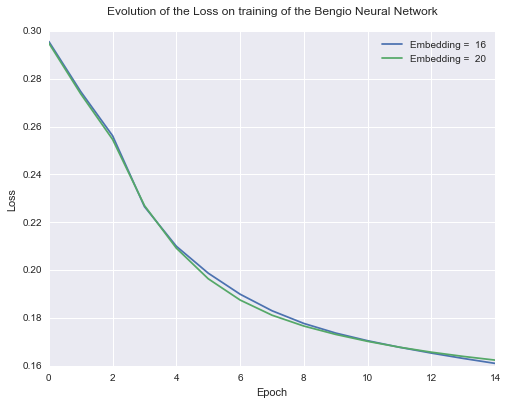
\includegraphics[width=1\linewidth]{train_nn_em}
  \caption{Training Loss}
\end{minipage}%
\begin{minipage}{.5\textwidth}
  \centering
  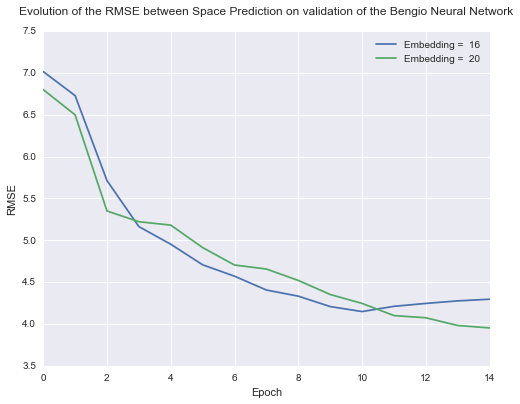
\includegraphics[width=1\linewidth]{rmse_em}
  \caption{RMSE on Validation set}
\end{minipage}
\end{figure}

If the losses on training are very similar, we observed that greater embedding dimension yield better results on the validation. We therefore submitted to Kaggle, results using the latter model trained on 20 epochs and obtained:

$$RMSE_{nn} = \sqrt{13.37} = 3.65$$

We then experimented with this model by assignment a space as the next prediction by using a threshhold instead of using argmax prediction. The ratio of spaces to characters in the training set being relatively little, by specifying a probability smaller than 0.5 above which we generate a space could help the performance of the greedy algorithm. We present results for a cutoff probability ranging from 0.2 to 0.5:

\begin{figure}[H]
\begin{center}
    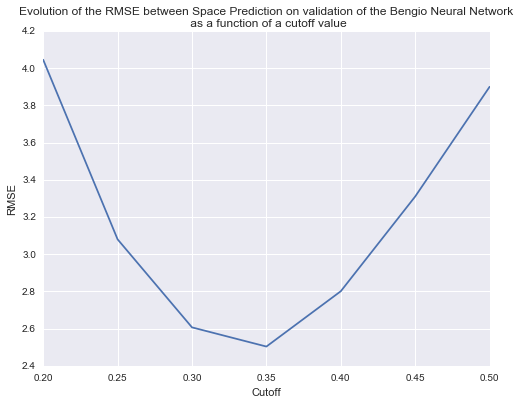
\includegraphics[width=0.5\textwidth]{cutoff}
    \caption{Perplexity evolution for the RNN}
\end{center}
\end{figure}

Results improve by 35\% using the cutoff trick, and the results on Kaggle are also much better:

$$RMSE_{cutoff} = \sqrt{6.09} = 2.47$$
\subsection{Recurrent Neural Networks}

For the three recurrent networks implemented, we have different parameters to take into account: 
\begin{itemize}
	\item batch size l
	\item length of sequences b
	\item embedding dimension emb
	\item number of epochs nEpochs
\end{itemize}

Choosing the right batch-size seems to be a tradeoff between performance and running time, a smaller one provides smaller perplexity but takes more time to run. The length of the sequence seems to provide good result when in the interval $[30,..,50]$ without significant peak so we kept values in this zone. We set the embedding dimension to 20 for the experiments with some prior explorations also.


\begin{figure}[H]
\begin{center}
    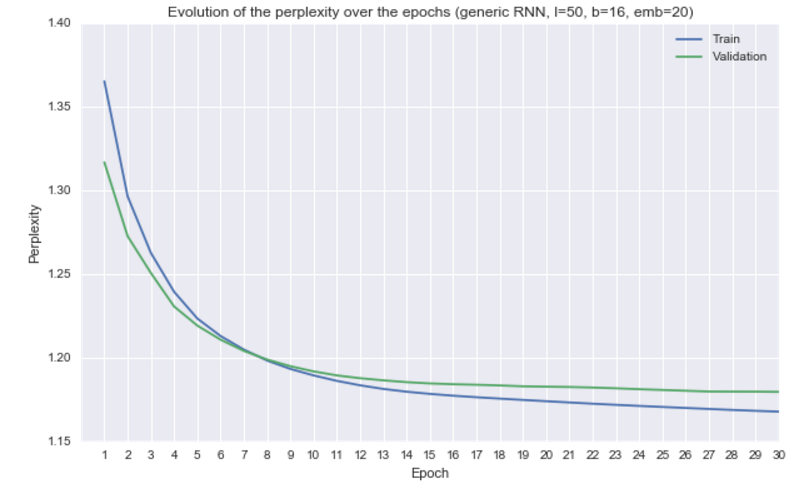
\includegraphics[width=0.45\textwidth]{perp_rnn.png}
    \caption{Perplexity evolution for the RNN}
\end{center}
\end{figure}

\begin{figure}[H]
\begin{center}
    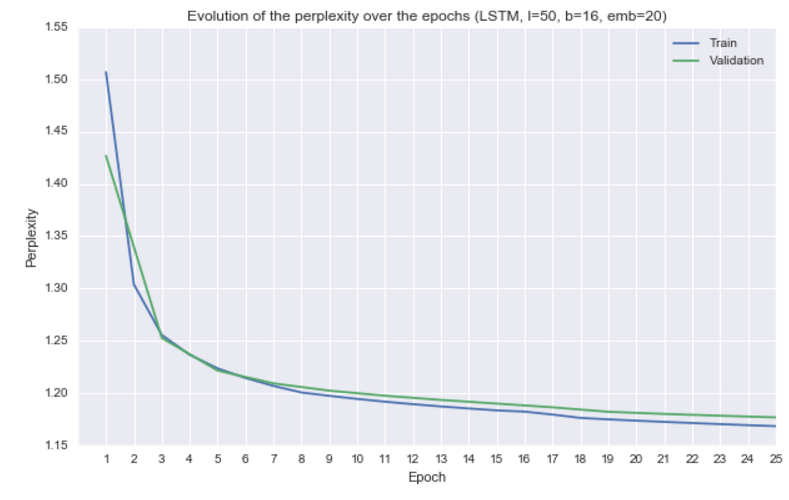
\includegraphics[width=0.45\textwidth]{perp_lstm.png}
    \caption{Perplexity evolution for the LSTM}
\end{center}
\end{figure}

\begin{figure}[H]
\begin{center}
    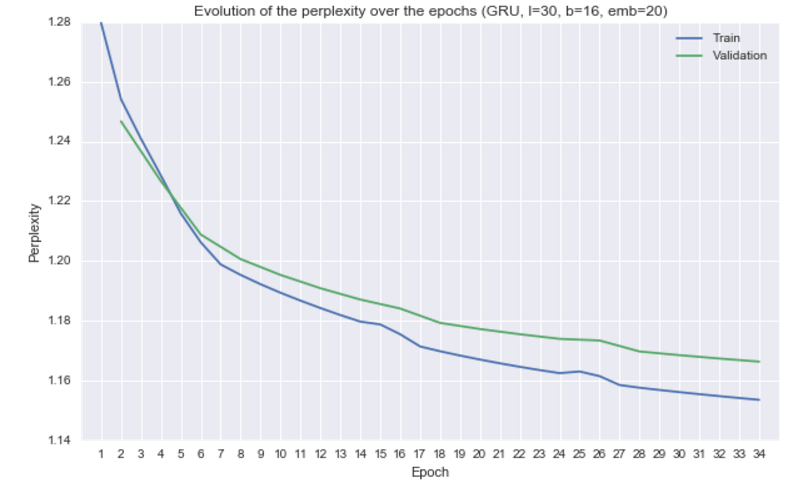
\includegraphics[width=0.45\textwidth]{perp_gru.png}
    \caption{Perplexity evolution for the GRU}
\end{center}
\end{figure}

The best results on the Kaggle were provided with the GRU after a large number of epochs (around 100).

We also applied the cutoff trick on the GRU to refine the sequence generation for the Kaggle competition. Here the metric we care about is the RMSE on the number of spaces per sentence. We tuned the cutoff value on the validation set. We kept the cutoff value reaching the minimum of RMSE for both the GRU (0.325) and the RNN (0.275) and combined them with a weighted sum to obtain our best result on Kaggle.

\begin{figure}[H]
\centering
\begin{minipage}{.5\textwidth}
  \centering
  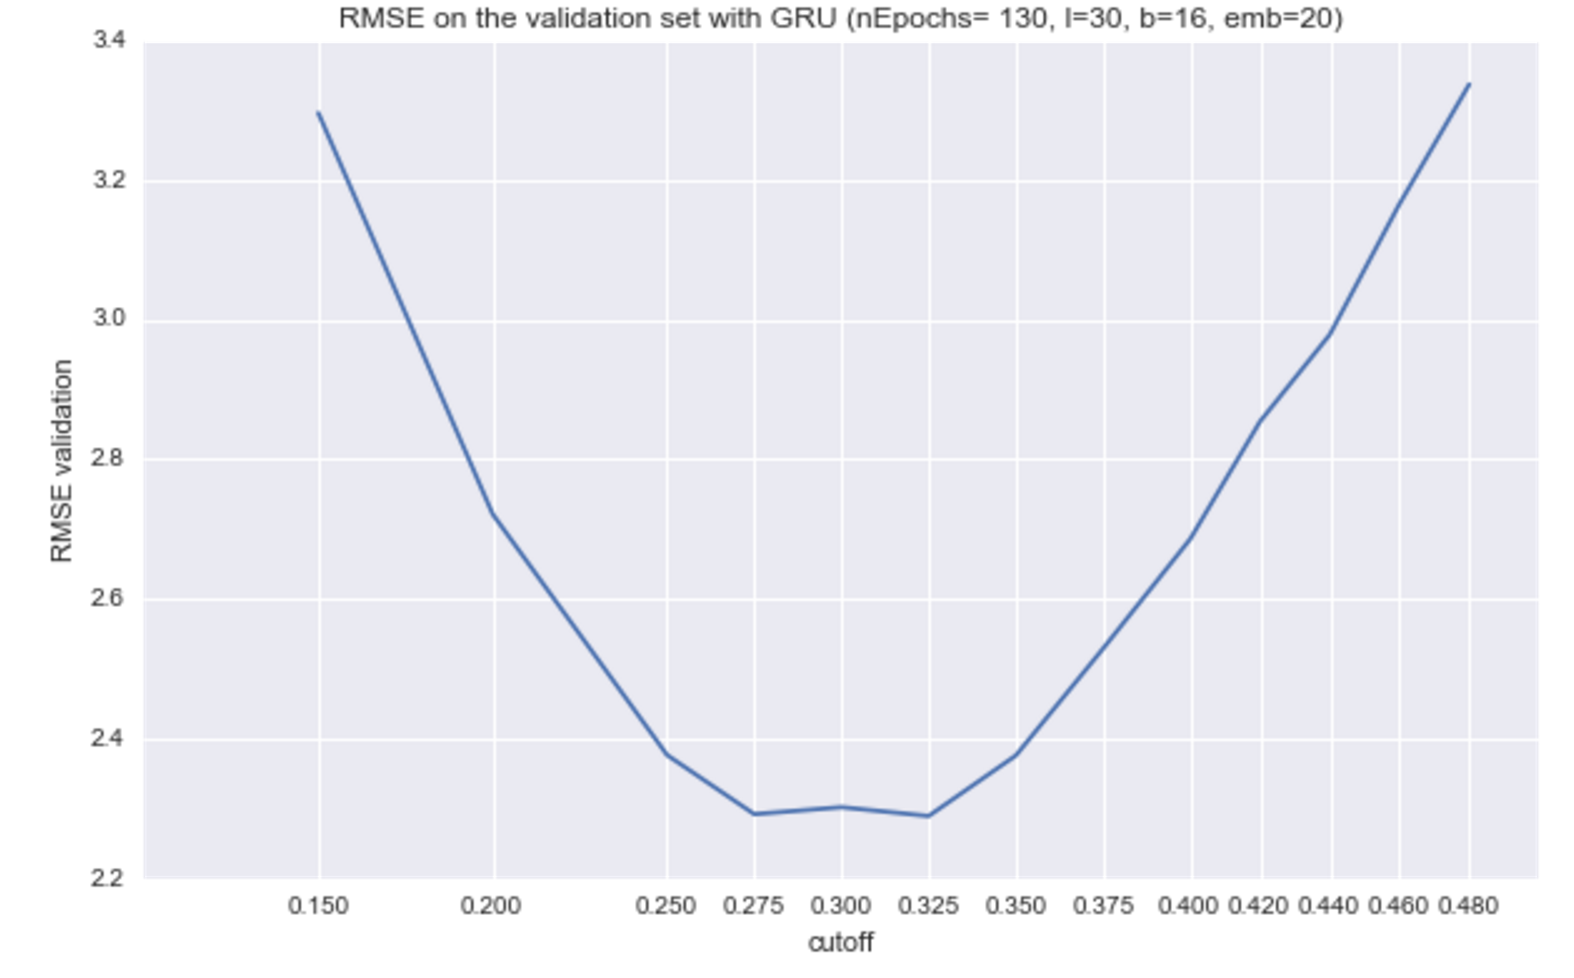
\includegraphics[width=1\linewidth]{gru_cutoff}
  \caption{RMSE on the validation with the GRU with cutoff}
\end{minipage}%
\begin{minipage}{.5\textwidth}
  \centering
  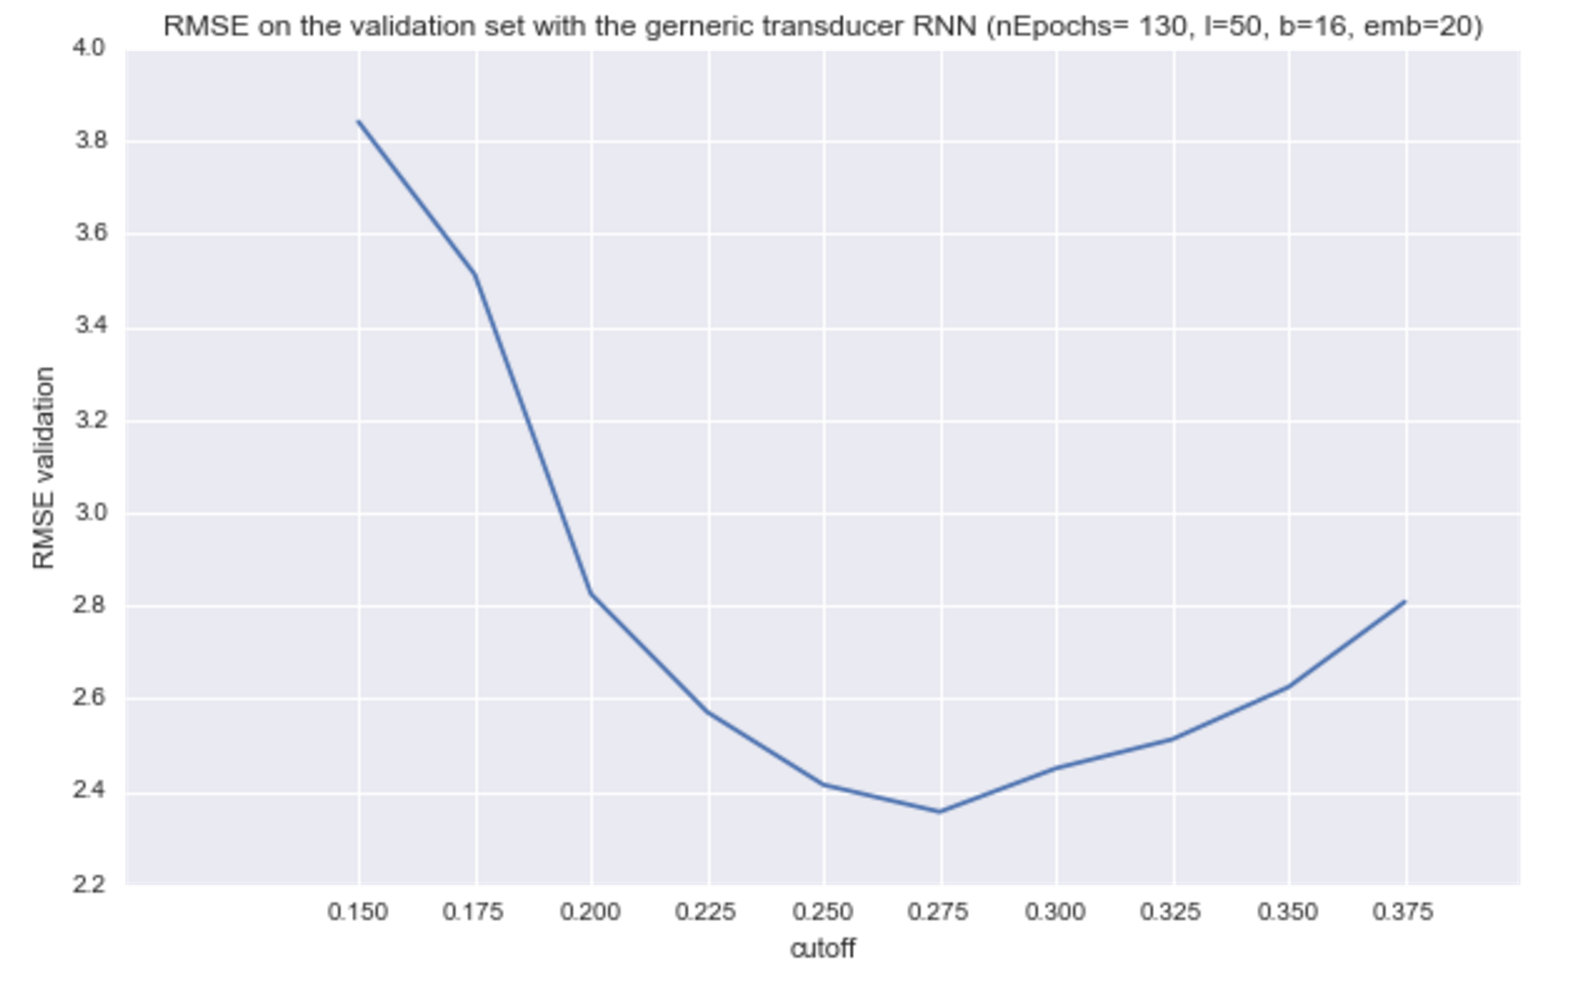
\includegraphics[width=1\linewidth]{rnn_cutoff}
  \caption{RMSE on the validation with the RNN with cutoff}
\end{minipage}
\end{figure}



\subsection{Model performance summary}

Here we summarize the performance of our different models. We reported the perplexity on the validation set computed from the model and the RMSE computed by Kaggle on the sequence predicted with our chosen algorithm.

First, we observed that the count 5gram count based model still provides a better sequence generated with the greedy algorithm as the 3gram one generated with Viterbi.
We also have a notable difference for the reccurent networks with the RMSE computed on Kaggle even though we have similar perplexity. The large value of RMSE on the validation could be decreased with an adaptive cutoff as we showed it for our best model.

\begin{table}[H]
\centering
\caption{Summary of the results}
\begin{tabular}{|l|l|l|l|}
\hline
Model             & Sequence generation algorithm & Perplexity on validation & MSE Kaggle \\ \hline
count based 5gram & Greedy                        & 1.1467                   & 17.88       \\ \hline
count based 3gram & Viterbi                       & 1.2780                   & 56.27       \\ \hline
NN                & Greedy                             & 1.156                        & 13.37926           \\ \hline
NN with cutoff               & Greedy                           &       1.156                  & 6.09           \\ \hline
RNN               & Greedy                        & 1.1746                   & 33.13       \\ \hline
LSTM              & Greedy                        & 1.1766                   & 18.95       \\ \hline
GRU               & Greedy                        & 1.1513                   & 10.94       \\ \hline
\textbf{GRU + RNN with cutoof}           & Greedy                        & -                  & \textbf{5.39}       \\ \hline
\end{tabular}
\end{table}


\section{Conclusion}

This segmentation task gave us the opportunity to implement different recurrent neural network architectures but also to compare them with more traditionnal method. Whereas the count based and even the simple neural network models are pretty fast to train they still provide interesting results. The results provided by the three variants of RNN were interesting to illustrate the influence of gates and memory in such networks. The gated reccurent network ended as the best model on this task. One future work could be to stack more layers to our reccurent architecture or to implement a network with a dynamic memory part to give more flexibility in how the model uses the information it already processed.



\begin{appendices}
\textbf{\huge\underline{Preprocessing:}}
\lstinputlisting[numbers=left, breaklines=true]{../preprocess.py}
\textbf{\huge\underline{Count-Based Models:}}
\lstinputlisting[numbers=left, breaklines=true]{../count_based.lua}
\textbf{\huge\underline{NNLM:}}
\lstinputlisting[numbers=left, breaklines=true]{../NeuralNetwork.lua}
\textbf{\huge\underline{RNN:}}
\lstinputlisting[numbers=left, breaklines=true]{../rnn.lua}
\end{appendices}
\end{document}
